\documentclass[titlepage, a4paper, 10pt]{article}

\usepackage{amssymb}
\usepackage{amsmath}
\usepackage{pgfplots}
\usepackage[margin=1in]{geometry}
\usepackage{fancyhdr}
\usepackage{xcolor}
\usepackage{array}
\usepackage{tikz}
\usepackage{booktabs}
\usepackage{bm}
\usetikzlibrary{positioning}

\title{\normalsize PLUS Session Worksheet \\[1em] \Large \textit{MATH 1554:} Linear Algebra}
\date{Fall 2023}
\author{\textit{Covering lessons}: 3.1 -- 3.3}

% ------- Set up header -------
\renewcommand{\sectionmark}[1]{\markright{#1}} % from https://tex.stackexchange.com/a/317393/227665
\pagestyle{fancy}
\fancyhead[L]{Fall 2023}
%\fancyhead[C]{\textit{\nouppercase{\rightmark}}}
\fancyhead[C]{\textit{Determinants and Transformations (3.1) -- (3.3)}}
\fancyhead[R]{\textbf{\thepage}}
% -------------------------------------------------------

% ------- Set up math stuff -------
\renewcommand{\vec}[1]{\bm{#1}}
\DeclareMathOperator{\vspan}{Span}
\DeclareMathOperator{\row}{row}
\DeclareMathOperator{\col}{col}
\DeclareMathOperator{\colspace}{Col}
\DeclareMathOperator{\nullspace}{Nul}
\DeclareMathOperator{\rank}{rank}
% -------------------------------------------------------

% ------- Set up Main Idea box environment -------
\newcounter{mainideas}
\setcounter{mainideas}{1}
\newcommand{\mainidea}{\textbf{Main Idea \#\themainideas \stepcounter{mainideas}}}
\setlength\fboxsep{1em}
%\newcommand{\midea}[2]{\begin{center}\fbox{\parbox{#1}{\centering \mainidea #2}} \end{center}} % Could be environment but I couldn't bother

% The way this works is that the savebox collects whatever was between the minipage and the end of it, then in the last line of the definition of the environment
% we regurgigate whatever was collected into an fbox which we center.
\newsavebox{\mybox}
\newenvironment{mideea}[1]
{%
\begin{lrbox}{\mybox}%
	\begin{minipage}{#1\textwidth}
		{\centering \mainidea \par}

}
{\end{minipage}\end{lrbox}\begin{center}\fbox{\usebox{\mybox}}\end{center}}
% -------------------------------------------------------

% ------- Set up question environment -------
\newcounter{question}
\setcounter{question}{1}
\newenvironment{newquestion}
{
	\noindent\textbf{Question \thequestion}
}
{
\stepcounter{question}
\par
}
% -------------------------------------------------------

% ------- Set up circle -------
\newcommand{\bubble}{\tikz[baseline=-0.625ex]\draw[radius=0.5em, fill=white] (0,0) circle;}
\newcommand{\dbubble}{\tikz[baseline=-0.625ex]\draw[radius=0.5em, fill=black] (0,0) circle;}
% -------------------------------------------------------

\begin{document}
    \maketitle

    \section{\centering T/F Questions}
        \begin{newquestion}
		Mark each statement \emph{true} if it's always true. Otherwise, mark it as \emph{false}.
		\begin{table}[!h]
			\centering
			\begin{tabular}{c@{\hspace{2.5em}}cp{0.8\textwidth}}
				true & false & \\
				\specialrule{\lightrulewidth}{0.25em}{1.25em}
			         \bubble & \bubble & For any square matrix \(AB\), \(\det(AB) = \det A \cdot \det B\).\\[0.75em]
				 \bubble & \bubble & If \(B\) is a \(n \times n\) matrix and \(\colspace B \ne \mathbb{R}^n\), then for any \(n \times n\) matrix \(A\), we
								have that \(\det(AB) = \det(B)\).\\[1.75em]
				\bubble & \bubble & Given that \(A\) is a square matrix and we obtain a matrix \(B\) by scaling a row of \(A\) by 2, then 
							      \(\det A = 2 \cdot \det B\). \\[1.75em]
				\bubble & \bubble & If \(\det(A^{2023}) = 5\), then \(A\) is non-singular. \\[0.75em]
				\bubble & \bubble & While the determinant of a lower triangular matrix is the product of it's diagonals, this is not the case for upper
							      triangular matrices. \\[1.75em]
				\bubble & \bubble & For a square matrix \(A\) that has an \(LU\)-factorization \(A = LU\), \(\det(A) = \det(U)\).\\[0.75em]
				\bubble & \bubble & Scaling a column of a square matrix by a factor of 2 doubles the determinant of the matrix.\\[0.75em]
				\bubble & \bubble & If \(A\) is an invertible matrix, then \(\displaystyle \det(A) = \frac{1}{\det(A^{-1})}\).\\[0.75em]
			\bottomrule
			\end{tabular}
		\end{table}

	\end{newquestion}

    \section{\centering Short Answer Questions}
    \begin{mideea}{0.9}
        \begin{enumerate}
            \item \(\det A = 0 \iff A \ \text{is not invertible}\).
            \item Scaling any row by a constant
            scales the determinant by the same
            amount.
            \item \(\det(AB) = \det A \cdot \det B\)
            \item \(\det A = \det A^T\)
        \end{enumerate}
    \end{mideea}

    \begin{newquestion}
        Use the statements in
        \textbf{Main Idea \#1} to answer the 
        following questions.

        \begin{enumerate}
            \item If \(
                \begin{vmatrix}
                    a & b & c \\
                    d & e & f \\
                    g & h & i
                \end{vmatrix} = 6
                \), what's \(
                \begin{vmatrix}
                    g &  2h & i \\
                    a &  2b & c \\
                    3d & 6e & 3f \\
                \end{vmatrix}
                \)?
            \item What's 
                \(\begin{vmatrix}
                    a & b & 2a + b \\
                    c & d & 2c + d \\
                    e & f & 2e + f
            \end{vmatrix}\)?
	    \item If \(\det(A^2 \cdot B^4) = 32\) and  \(\det(A) = \sqrt{2}\), find \(\det B\). (Note that \(A, B \in \mathbb{R}^n\).)
	    \item The matrix \(B\) was obtained by scaling the matrix \(C\) by a factor of 2, were \(C\) is a \(n \times n\). Then, the matrix \(A\) was obtained by
		     swapping 2 rows of \(B\). Given that \(\det A = 24\), what is \(\det C\)?
	    \item What value of \(k\) will cause the matrix \[\begin{bmatrix}1 & 14 & 2 \\ 0 & k & 3 \\ 1 & 2 & 0\end{bmatrix}\] to be singular?
            \item[\textbf{*}] What's the area of the 
                  parallelogram whose vertices 
                  are \((0, 0), (1, 2), (3, 1), (4, 3)\)? What's the area after
                  applying the mapping \(\vec{x} \mapsto \begin{bmatrix}
                      3 & 0 \\ 0 & 1
                  \end{bmatrix}\vec{x}\) on
                  the vertices?
        \end{enumerate}
    \end{newquestion}

\section{\centering Solutions}

\subsection{Solution to T/F Questions}
		\begin{table}[!h]
			\centering
			\begin{tabular}{c@{\hspace{2.5em}}cp{0.8\textwidth}}
				true & false & \\
				\specialrule{\lightrulewidth}{0.25em}{1.25em}
			         \bubble & \dbubble & For any square matrix \(AB\), \(\det(AB) = \det A \cdot \det B\).\\[0.75em]
				 \dbubble & \bubble & If \(B\) is a \(n \times n\) matrix and \(\colspace B \ne \mathbb{R}^n\), then for any \(n \times n\) matrix \(A\), we
								have that \(\det(AB) = \det(B)\).\\[1.75em]
				\bubble & \dbubble & Given that \(A\) is a square matrix and we obtain a matrix \(B\) by scaling a row of \(A\) by 2, then 
							      \(\det A = 2 \cdot \det B\). \\[1.75em]
				\dbubble & \bubble & If \(\det(A^{2023}) = 5\), then \(A\) is non-singular. \\[0.75em]
				\bubble & \dbubble & While the determinant of a lower triangular matrix is the product of it's diagonals, this is not the case for upper
							      triangular matrices. \\[1.75em]
				\dbubble & \bubble & For a square matrix \(A\) that has an \(LU\)-factorization \(A = LU\), \(\det(A) = \det(U)\).\\[0.75em]
				\dbubble & \bubble & Scaling a column of a square matrix by a factor of 2 doubles the determinant of the matrix.\\[0.75em]
				\dbubble & \bubble & If \(A\) is an invertible matrix, then \(\displaystyle \det(A) = \frac{1}{\det(A^{-1})}\).\\[0.75em]
			\bottomrule
			\end{tabular}
		\end{table}

\subsection{Solution to Short Answer Questions}
\begin{enumerate}
	\item 36.
	\item 0.
	\item 2.
	\item \(-24/2^n\).
	\item \(k = 18\). You do this problem through setting the determinant to 0 and finding the value \(k\) that does this.
	\item First, a picture.
		\begin{figure}[!h]
			\centering
			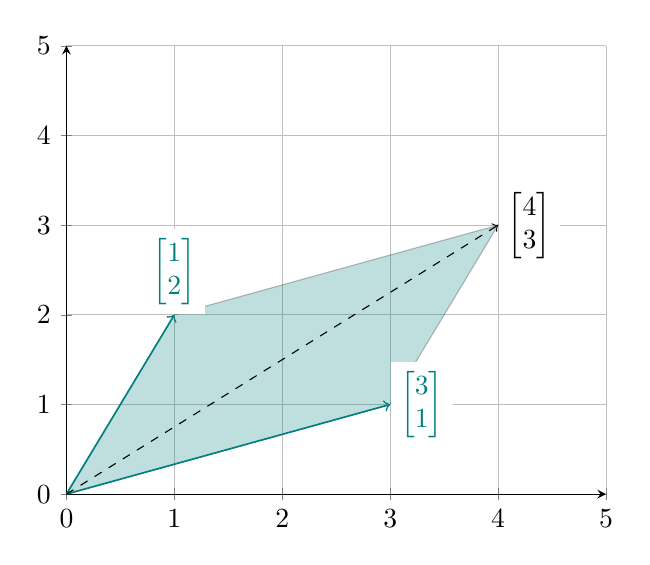
\begin{tikzpicture}
				\begin{axis}[axis lines=left, xmin=0, xmax=5, ymin=0, ymax=5,grid=major]
					\draw[fill=teal, opacity=0.25] (axis cs:0,0) -- (axis cs:1,2) -- (axis cs:4,3) -- (axis cs:3,1)  -- (axis cs:0,0);
					\addplot[->, semithick, domain=0:1, color=teal] {2*x} node[above, fill=white] {\(\begin{bmatrix}1 \\ 2\end{bmatrix}\)};
					\addplot[->, semithick, domain=0:3, color=teal] {1/3*x} node[right, fill=white] {\(\begin{bmatrix}3 \\ 1\end{bmatrix}\)};
					\addplot[->, dashed, domain=0:4] {3/4 * x} node[right, fill=white] {\(\begin{bmatrix}4 \\ 3\end{bmatrix}\)};
				\end{axis}
			\end{tikzpicture}
			\caption{Pictorial representation of the problem.}
		\end{figure}
		\begin{enumerate}
			\item The signed area of this shape is the determinant of the matrix \(\begin{bmatrix}1 & 3 \\ 2 & 1\end{bmatrix}\). We find that the
			 	 determinant is \(-5\). The area is therefore 5.
			\item We \emph{could} apply the transformation on each point and find the determinant of a new matrix, but a simpler way is to rely on the formula
				\[V_T = V_S \cdot \lvert \det A \rvert.\]
				Applying the above formula, we get that \(V_T\) (the volume of the transformed shape) is equal to \(V_S\) (the original volume) times
				\(\lvert \det A \rvert = 3.\) So, \(V_T = 15\).
		\end{enumerate}
\end{enumerate}

\end{document}